\renewcommand{\newCommandChapterTitle}{Extracción de \textit{features} en el contexto HTTP}
\chapter{\newCommandChapterTitle}
\markright{\hfill \thechapter. \newCommandChapterTitle}
\label{chap:p3_concepts_features}


La extracción de \textit{features} consiste en obtener características
representativas de los datos originales
\citep{torranoGimenez2015study}. % from section 2.3.1 - feature extraction
En nuestro caso, las características de los mensajes \gls{acr3:http} deben
ser expresadas por medio de vectores numéricos para que los clasificadores
\gls{acr3:ocsvm} del \gls{acr3:name} puedan reconocer dichas características.
En \citep{rieck2009machine} % from section 2.2 - feature maps
se habla también de mapas de \textit{features} para referirse a esta
extracción de características; se presenta este proceso como funciones
que mapean el dominio de mensajes \gls{acr3:http} a un espacio vectorial
$\mathbb{R}^{n}$ de números reales, donde $1 \leq n \leq \infty$.

En este capítulo, en primer lugar damos algunas explicaciones sobre
la estructura de los mensajes \gls{acr3:http}, luego presentamos los
aportes de los trabajos de Kruegel y Vigna sobre las características
que utilizaron, y finalmente describimos los procesos de extracción de
\textit{features} que utiliza \gls{acr3:name} para realizar el mapeo de
mensajes a vectores numéricos.


\section{Estructura de mensajes HTTP}

El detector \gls{acr3:name} que presentamos en este trabajo analiza
mensajes \gls{acr3:http} y en esta sección introducimos los conceptos
necesarios sobre este protocolo de comunicación.
Nosotros solamente nos enfocamos en el protocolo \gls{acr3:http} en su
versión 1.1, en el cual los mensajes son enviados en formato de texto
\citep{fielding1999http}. % from the abstract

Además, \gls{acr3:name} analiza solamente los mensajes \gls{acr3:http}
que sean peticiones, ignorando los mensajes que sean respuestas. Debido
a que las peticiones son aquellos mensajes que llegan a las aplicaciones
web desde la Internet, estos pueden contener ataques; en cambio, los
mensajes de respuesta son generadas por las aplicaciones protegidas por
el \gls{acr3:waf} y por lo tanto hay menos riesgos de seguridad.
Obviando el análisis de las respuestas reducimos el procesamiento necesario
sin aumentar de forma significativa el riesgo de ataques.

Las peticiones \gls{acr3:http} pueden estar compuestas por seis partes:
un método \gls{acr3:http}, un identificador universal de recursos
(\gls{acr3:url} - \textit{Universal Resource Locator}), un \textit{query string},
la versión del protocolo, varias cabeceras y finalmente el cuerpo de la
petición \citep{fielding1999http}. % from section 5 - request
El método debe ser uno de los valores definidos para el protocolo; nuestro
\gls{acr3:waf} se enfoca solamente en peticiones con los métodos GET y POST,
ya que estos son los más utilizados.
La \gls{acr3:url} está compuesta por el indicador de protocolo, la dirección
del \textit{host}, el puerto y la ruta del recurso pedido (\textit{path}).
Las cabeceras son opcionales y permiten enviar información adicional sobre
la petición. Cada cabecera consiste en un nombre y su valor, separados por
el signo de dos puntos (:). Las cabeceras van delimitadas por los caracteres
de nueva linea (CRLF).

El \textit{query string}, que es opcional, va separado de la \gls{acr3:url}
mediante un signo de interrogación (?) y está compuesto por pares de
parámetros y valores. Estos parámetros están separados de sus valores
mediante el símbolo de igualdad (=), mientras que los pares se encuentran
delimitados por el símbolo \textit{ampersand} (\&). De esta forma, el
\textit{query string} de una petición puede ser representado como la lista
de pares ordenados
$\{ (p_{1}, v_{1}), (p_{2}, v_{2}), \dots , (p_{n}, v_{n}) \}$.
Estos parámetros son utilizados, por ejemplo, para pasar criterios de
filtrado y ordenación de datos a las aplicaciones.

Las peticiones del método GET no suelen llevar un cuerpo. Las peticiones
del método POST en algunos casos lo tienen, y en caso de contar con el
mismo, su contenido puede estar estructurado de varias formas posibles.
Para esta investigación consideramos únicamente los cuerpos de peticiones
POST que constan de pares de parámetros y valores estructurados de la
misma forma que el \textit{query string}. De esta manera, el cuerpo de
una petición puede ser expresado como la lista
$\{ (p_{1}, v_{1}), (p_{2}, v_{2}), \dots , (p_{n}, v_{n}) \}$.
En esta investigación, no analizamos cuerpos de peticiones con contenido
en otros formatos, por ejemplo aquellos que tengan datos binarios.
Los cuerpos de peticiones POST pueden ser utilizados, por ejemplo, para
enviar datos de formularios completados por usuarios a aplicaciones web.

\begin{figure}[htb]
    \centering
    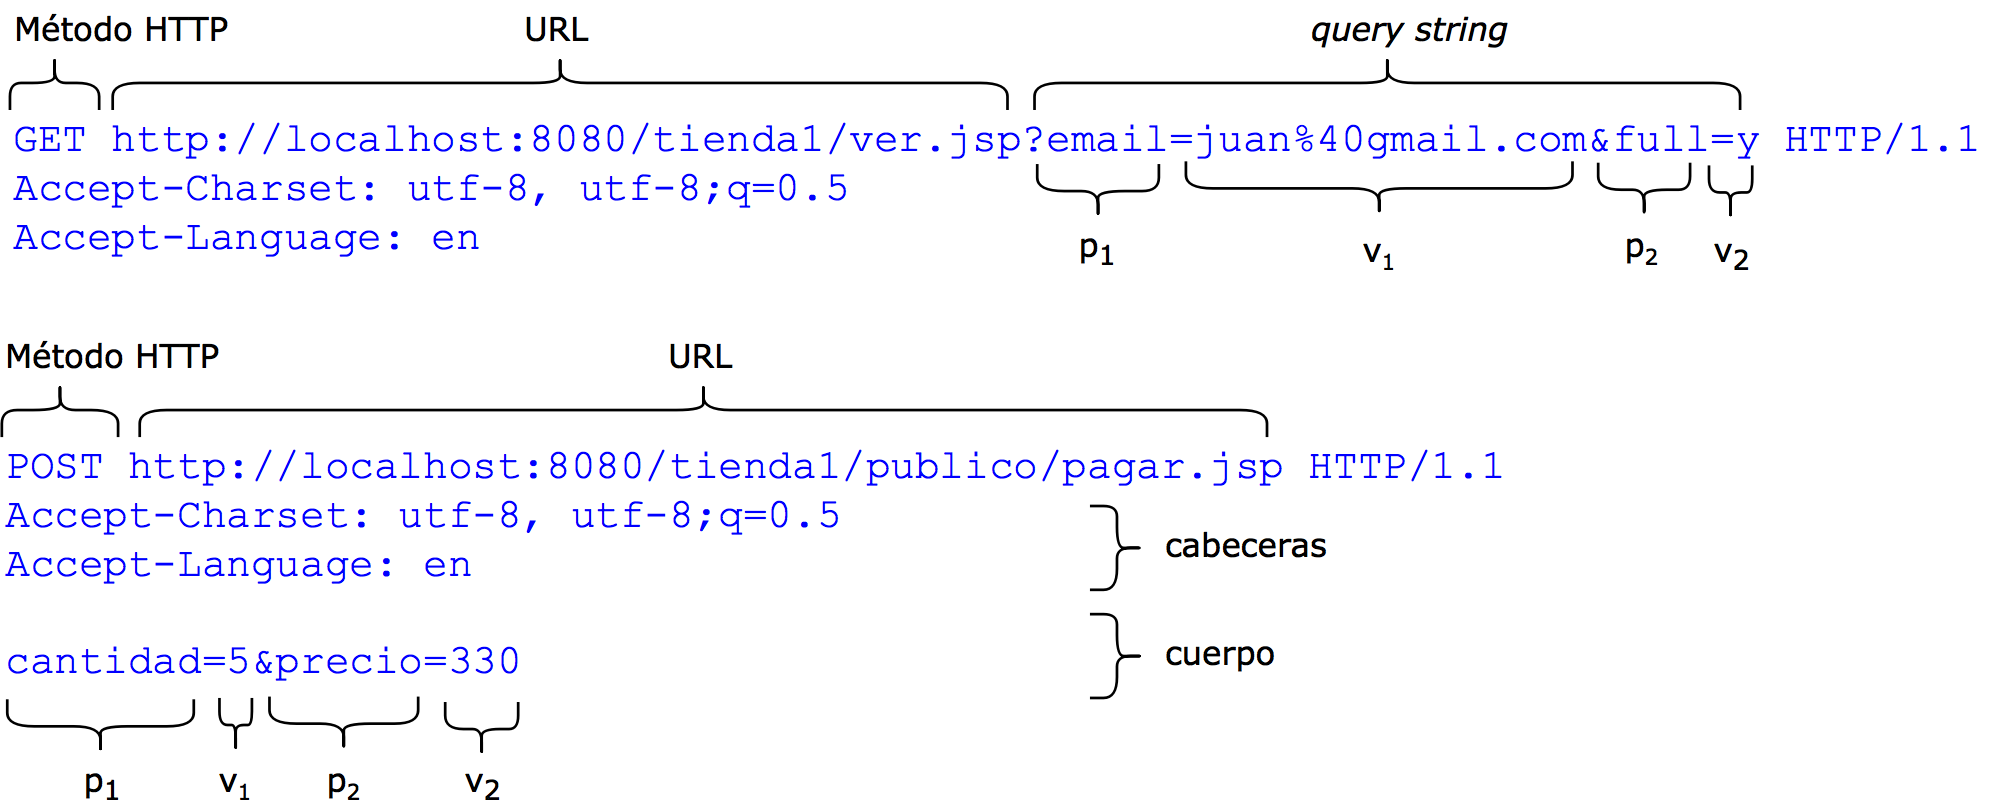
\includegraphics[width=\linewidth]{images/http-request-structure.png}

    \caption{Diagrama de estructura de dos peticiones \gls{acr3:http},
        una con método GET y otra con método POST.}
    \label{fig:fe:http_request_structure}
\end{figure}

En la \autoref{fig:fe:http_request_structure} se puede observar la estructura
de dos peticiones de ejemplo. La primera es una petición con el método GET.
La misma tiene un \textit{query string} con los dos parámetros \textit{email}
y \textit{full} con sus respectivos valores. Esta primera petición no
tiene cuerpo. La segunda petición tiene el método POST y no cuenta con un
\textit{query string}, pero en el cuerpo contiene los parámetros \textit{modo}
y \textit{precio} con sus valores. Ambas peticiones contienen dos cabeceras
que son \textit{Accept-Charset} y \textit{Accept-Language} con sus valores.
Cabe mencionar que los caracteres de la petición que tienen significado
especial en el contexto del mensaje deben ser reemplazados por un código
hexadecimal precedido por un símbolo de porcentaje (\%), un proceso conocido
como \textit{percent encoding}
\citep{bernerslee2005uri}. % from section 2.1 - percent encoding
Este reemplazo se puede observar en el valor del parámetro \textit{email}
de la primera petición de la figura mencionada, donde el símbolo @ queda
reemplazado por el código \%40.


\section{Características HTTP según Kruegel y Vigna}

Los autores Kruegel y Vigna presentaron varias ideas relacionadas a la
detección de anomalías en peticiones \gls{acr3:http}.
En los trabajos \citep{kruegel2003anomaly} y \citep{kruegel2005multi}
utilizan conocimiento experto sobre mensajes \gls{acr3:http},
específicamente sobre las peticiones, para construir modelos de anomalías
durante una fase de entrenamiento y luego, durante una fase de detección,
emplean esos modelos para obtener una detección eficaz.
Nosotros basamos nuestra propuesta en dos aspectos de sus aportes:
en primer lugar usamos el análisis de valores de parámetros del
\textit{query string} que ellos proponen y en segundo lugar empleamos
algunas de las características que ellos utilizan en sus modelos de
anomalías.

Cabe mencionar que Kruegel y Vigna utilizan métodos estadísticos para
la detección de anomalías y no herramientas de \gls{acr3:ml} como nosotros.
Debido a eso, ellos no utilizan vectores de \textit{features}.
Aun así, utilizamos los dos aspectos de sus aportes mencionados anteriormente
para mejorar nuestros procesos de extracción de \textit{features}, apuntando
a mejorar la detección de peticiones anómalas del \gls{acr3:name}.
Adicionalmente, Kruegel y Vigna realizan sus tareas de detección de
anomalías en base a archivos \textit{logs} de servidores \gls{acr3:http},
pero no trabajan sobre tráfico en tiempo real. Como en esos \textit{logs}
solamente había peticiones con el método GET, sus trabajos tratan únicamente
de ese tipo de peticiones.


\subsection{Análisis de valores de parámetros}

Los autores Kruegel y Vigna aplican sus modelos de anomalías sobre el
\textit{query string} de peticiones GET y además sobre los valores individuales
de los parámetros de la misma. En la fase de detección, sus modelos obtienen
una probabilidad de que el valor analizado pertenezca al conjuntos de valores
vistos durante el entrenamiento.

Durante la fase de entrenamiento, en primer lugar las peticiones
\gls{acr3:http} son agrupadas por método y \gls{acr3:url}; los autores
utilizaron solamente peticiones GET y así en la práctica su agrupación
fue por \gls{acr3:url} únicamente.
Esta agrupación se realiza ya que peticiones que van dirigidas a una misma
\gls{acr3:url} y con el mismo método \gls{acr3:http} presentan más
similitudes entre ellas que con peticiones que tienen otro método o
\gls{acr3:url}. De esta manera, se obtiene modelos de anomalías
independientes y más precisos dentro de cada grupo.
Después de agrupar, se realiza la extracción de los parámetros que aparecen
en el \textit{query string} de las peticiones dentro de cada grupo. Luego
se construye modelos de anomalías por cada uno de los parámetros extraídos,
utilizando los valores que dichos parámetros tienen en las peticiones del
conjunto de entrenamiento.
Por ejemplo, se analiza la longitud de todos los valores de un parámetro,
construyendo de esta forma un modelo de anomalía que utiliza promedio
y desviación estándar de las longitudes para definir a partir de qué
longitud un valor de ese parámetro específico será considerado anómalo.
Además, se tiene modelos aplicados al \textit{query string} completo,
como por ejemplo el análisis de presencia de parámetros.

Durante la fase de detección, el sistema propuesto por los autores
mencionados analiza las peticiones nuevas con los modelos construidos
previamente. Primeramente se busca el grupo al cual pertenece la petición,
luego se obtiene la lista de parámetros vistos durante el entrenamiento
para ese grupo y luego se extraen todos los valores que esos parámetros
tienen en la petición en cuestión. Después se aplican los modelos sobre
los valores, obteniendo resultados que indican la probabilidad de que
los nuevos valores sean normales.
Así, por cada parámetro de la petición se tendrá varios resultados calculados
por los distintos modelos, de los cuales se obtiene una probabilidad final
mediante una suma ponderada. Esta probabilidad final es comparada con un
umbral (\textit{threshold}) establecido previamente para decidir si la
petición analizada es normal o anómala.

En esta parte cabe resaltar que el análisis hecho por estos autores utiliza
una cantidad variable de modelos en cada grupo de peticiones, ya que cada
grupo puede tener una cantidad distinta de parámetros; esa cantidad de
parámetros observados durante el entrenamiento determina la cantidad de
modelos que se tendrá.
Este abordaje es diferente a otros trabajos relacionados al área de
\gls{acr3:ids} en donde se utiliza una cantidad fija de características
de los mensajes; podemos ver un ejemplo de esto en
\citep{nguyen2011application}, % from section 3 - experiments
donde se utiliza 30 \textit{features} de peticiones \gls{acr3:http}
para los distintos clasificadores empleados.


\subsection{Características analizadas de los mensajes}

Kruegel y Vigna analizan un total de nueve características distintas
en sus trabajos \citep{kruegel2003anomaly} y \citep{kruegel2005multi},
a partir de las cuales construyen sus modelos de anomalías; estas
características pueden ser observadas en la
\autoref{tbl:fe:kruegel_feature_list}.

Los autores detallan también los tipos de ataques que se busca detectar
con cada uno de sus modelos de anomalías. Entre los ataques detectados se
encuentran, por ejemplo, ataques de \textit{buffer overflow},
\textit{directory transversal}, \textit{cross-site scripting}
y también \textit{SQL injection}.

\begin{table}[ht]
    \centering
    \small
    \begin{tabularx}{\linewidth}{|X|c|}
        \hline
        \multicolumn{1}{|c|}{Características analizadas por Kruegel y Vigna}
        & Características utilizada en \gls{acr3:name} \\
        \specialrule{1.5pt}{0}{0}
        Longitud                            & Sí \\ \hline
        Distribución de caracteres          & Sí \\ \hline
        Inferencia de estructura            & -  \\ \hline
        Análisis de \textit{tokens}         & -  \\ \hline
        Presencia o ausencia de parámetros  & -  \\ \hline
        Orden de parámetros                 & -  \\ \hline
        Frecuencia de invocación            & -  \\ \hline
        Tiempo entre invocaciones           & -  \\ \hline
        Orden de invocación                 & -  \\ \hline
    \end{tabularx}

    \caption{Características de mensajes \gls{acr3:http} utilizadas por
        Kruegel y Vigna en sus modelos de anomalías, indicando también
        cuales de estas características son utilizadas en \gls{acr3:name}.}
    \label{tbl:fe:kruegel_feature_list}
\end{table}

En nuestra opinión, no todas las características presentadas son aplicables
a nuestro caso con herramientas de \gls{acr3:ml}. De esa forma, nosotros
empleamos solamente dos de las características de la tabla mencionada para
construir los procesos de extracción de \textit{features} del \gls{acr3:name};
estos procesos son presentados en la siguiente sección.


\section{Nuestros procesos de extracción de \textit{features}}

En esta sección presentamos los procesos que realizan la extracción de
\textit{features} en \gls{acr3:name}. Primeramente, describimos la agrupación
de peticiones que realizamos, luego explicamos el análisis de valores de
parámetros que hacemos y después detallamos los \textit{features} que
extraemos de cada uno de los valores.

A modo de ilustrar mejor los conceptos de esta sección, utilizamos un
conjunto de peticiones de ejemplo sobre el que aplicamos nuestros procesos
de extracción que presentamos a continuación. En la \autoref{tbl:fe:example_1}
se pueden observar dichas peticiones de ejemplo, que son 20 peticiones GET
que fueron hechas a una misma \gls{acr3:url}. De este conjunto, las primeras
15 peticiones son normales y las otras 5 contienen alguna anomalía o ataque.
Además, las primeras 10 peticiones normales serán utilizadas para la fase
de entrenamiento, mientras que las demás normales y las anomalías recién
serán utilizadas para la fase de detección.

\begin{table}[!th]
    \centering
    \fontsize{10}{12}\selectfont
    \begin{tabularx}{\linewidth}{|c|C|C|>{\ttfamily}l|}
        \hline
        ID & Clase    & Grupo         & \multicolumn{1}{c|}{Petición completa}                       \\
        \specialrule{1.5pt}{0}{0}
         1 & normal   & entrenamiento & GET http://localhost:8080/tienda1/miembros/ver.jsp?          \\
           &          &               & email=talmadge\%40movintel.uz HTTP/1.1                       \\ \hline
         2 & normal   & entrenamiento & GET http://localhost:8080/tienda1/miembros/ver.jsp?          \\
           &          &               & email=tarangelo\%40accesoabierto.st HTTP/1.1                 \\ \hline
         3 & normal   & entrenamiento & GET http://localhost:8080/tienda1/miembros/ver.jsp?          \\
           &          &               & email=tarasova\_dabo\%40comerciosdeaspe.ly HTTP/1.1          \\ \hline
         4 & normal   & entrenamiento & GET http://localhost:8080/tienda1/miembros/ver.jsp?          \\
           &          &               & email=tazaki\_waggenheim\%40telelujo.an HTTP/1.1             \\ \hline
         5 & normal   & entrenamiento & GET http://localhost:8080/tienda1/miembros/ver.jsp?          \\
           &          &               & email=tati\%40callalabocaatiaherminia.travel HTTP/1.1        \\ \hline
         6 & normal   & entrenamiento & GET http://localhost:8080/tienda1/miembros/ver.jsp?          \\
           &          &               & email=tauber5\%40lamolahotel.bb\&full=yes HTTP/1.1           \\ \hline
         7 & normal   & entrenamiento & GET http://localhost:8080/tienda1/miembros/ver.jsp?          \\
           &          &               & email=tayo\%4013horas.tn HTTP/1.1                            \\ \hline
         8 & normal   & entrenamiento & GET http://localhost:8080/tienda1/miembros/ver.jsp?          \\
           &          &               & email=tanimoto\_hassen\%40autobuses-hibridos.tw HTTP/1.1     \\ \hline
         9 & normal   & entrenamiento & GET http://localhost:8080/tienda1/miembros/ver.jsp?          \\
           &          &               & email=tarp\%40redstarz.asia\&full=yes HTTP/1.1               \\ \hline
        10 & normal   & entrenamiento & GET http://localhost:8080/tienda1/miembros/ver.jsp?          \\
           &          &               & email=teje-lipman\%40hojainformativas.sa HTTP/1.1            \\ \hline
        11 & normal   & detección     & GET http://localhost:8080/tienda1/miembros/ver.jsp?          \\
           &          &               & email=taneda\%40ajuntamentdebcn20.be HTTP/1.1                \\ \hline
        12 & normal   & detección     & GET http://localhost:8080/tienda1/miembros/ver.jsp?          \\
           &          &               & email=tannen\%40getgold.ua HTTP/1.1                          \\ \hline
        13 & normal   & detección     & GET http://localhost:8080/tienda1/miembros/ver.jsp?          \\
           &          &               & email=tchjan-lian.quadflieg\%40comerciosdeaspe.se HTTP/1.1   \\ \hline
        14 & normal   & detección     & GET http://localhost:8080/tienda1/miembros/ver.jsp?          \\
           &          &               & email=tarver\%40callofduty6.lb\&full=yes HTTP/1.1            \\ \hline
        15 & normal   & detección     & GET http://localhost:8080/tienda1/miembros/ver.jsp?          \\
           &          &               & email=tay\%40autobuses-hibridos.ps HTTP/1.1                  \\ \hline
        16 & anomalía & detección     & GET http://localhost:8080/tienda1/miembros/ver.jsp?          \\
           &          &               & email=\%27\%3B+DROP+TABLE+user\%3B+SELECT+*+FROM+p+WHERE+    \\
           &          &               & name+LIKE+\%27\%25 HTTP/1.1                                  \\ \hline
        17 & anomalía & detección     & GET http://localhost:8080/tienda1/miembros/ver.jsp?          \\
           &          &               & email=malformed1email2address3domain4 HTTP/1.1               \\ \hline
        18 & anomalía & detección     & GET http://localhost:8080/tienda1/miembros/ver.jsp?          \\
           &          &               & email=tayo\_1\%4013horas.tn\&full=12345\&show=no HTTP/1.1    \\ \hline
        19 & anomalía & detección     & GET http://localhost:8080/tienda1/miembros/ver.jsp?          \\
           &          &               & email=\%3C\%21--\%23exec+cmd\%3D\%22cat+\%2Fetc\%2Fpasswd+   \\
           &          &               & \%3E+somefile\%22+--\%3E HTTP/1.1                            \\ \hline
        20 & anomalía & detección     & GET http://localhost:8080/tienda1/miembros/ver.jsp?          \\
           &          &               & email=\%40cr\%40anh\%40am\%404horas.ki\&full=yes HTTP/1.1    \\ \hline
    \end{tabularx}

    \caption{Conjunto de 20 peticiones \gls{acr3:http} de ejemplo utilizadas
        para ilustrar el funcionamiento de \gls{acr3:name} en este trabajo.}
    \label{tbl:fe:example_1}
\end{table}


\subsection{Agrupación de peticiones}

Basado en los trabajos de Kruegel y Vigna mencionados en la sección
anterior, \gls{acr3:name} también realiza la agrupación de las peticiones
\gls{acr3:http} por método y \gls{acr3:url}. De esta forma, a partir de
las peticiones utilizadas para el entrenamiento, \gls{acr3:name} crea
un conjunto \gls{sim3:g} de grupos de peticiones, que contiene todos
los grupos de peticiones obtenidos mediante la agrupación de los datos
de entrenamiento.

Con esta agrupación podemos lograr una descripción más precisa de las
peticiones normales dentro de cada grupo \gls{sim3:gi}. Esto posibilita
inclusive la identificación de aquellas peticiones que, por ejemplo, son
anómalas dentro de su grupo correspondiente $G_{1}$, pero que podrían ser
consideradas normales en el contexto de otro grupo $G_{2}$.

En el caso de nuestras 20 peticiones de ejemplo, todas ellas fueron hechas
con el método GET a una sola \gls{acr3:url}. Por lo tanto, dichas peticiones
pertenecen al mismo grupo. Cabe volver a mencionar que para el entrenamiento
utilizamos las 10 primeras peticiones normales.


\subsection{Extracción de valores de los parámetros del \textit{query string}
    y cuerpo de las peticiones}

Con la agrupación realizada, partimos de la base de que las peticiones
dentro de un grupo \gls{sim3:gi} presentan gran similitud entre ellas.
Específicamente, se espera que esas peticiones tengan los mismos parámetros
en \textit{query string} y cuerpo, o que por lo menos no haya mucha
variación. Por ejemplo, en una \gls{acr3:url} para inicio de sesión,
todas las peticiones con el método POST deberían contener los parámetros
\textit{username} y \textit{password} en su cuerpo.

Como ya se mencionó en la sección anterior, Kruegel y Vigna utilizan
solamente peticiones GET en sus trabajos. \gls{acr3:name} incluye el
análisis de parámetros del cuerpo de las peticiones POST.
Cabe mencionar que estamos conscientes del riesgo de seguridad que puede
presentar el hecho de que se analice el cuerpo de peticiones POST, ya
que los mismos pueden contener información confidencial, como por ejemplo
contraseñas de acceso de usuarios. Para ajustarse a las necesidades de
las distintas situaciones, \gls{acr3:name} puede ser configurado para
excluir ciertos métodos \gls{acr3:http} o ciertas \gls{acr3:url}s del
análisis que realiza. Estas configuraciones quedan a cargo de los
administradores del \gls{acr3:name}.

De esta forma, en la fase de entrenamiento se construyen listas de todos
los parámetros que aparecen en las peticiones \gls{acr3:http} dentro
de cada grupo. La lista \gls{sim3:qi} contiene de forma ordenada todos
los parámetros que aparecen en el \textit{query string} de alguna
petición dentro del grupo \gls{sim3:gi}, excluyendo las duplicaciones.
De forma análoga, la lista \gls{sim3:bi} contiene los parámetros que
aparecen en el cuerpo de alguna petición del grupo.
Es posible que estas listas queden vacías para un grupo, lo que sucede
cuando ninguna petición contiene parámetros. En nuestras 10 peticiones
de ejemplo para el entrenamiento, \gls{sim3:qi} contiene los dos parámetros
\textit{email} y \textit{full}, pero \gls{sim3:bi} queda vacío porque las
peticiones no tienen cuerpo con parámetros.
Como ya mencionamos, se espera que los mismos parámetros se repitan en la
mayoría de las peticiones, de manera que estas listas de parámetros de un
grupo no sean mucho más extensas que la cantidad de parámetros de una sola
petición de dicho grupo.

Después de construir estas listas, se procesan las peticiones de cada
grupo \gls{sim3:gi} para construir los conjuntos de vectores \gls{sim3:fi},
en donde cada petición está representada por un vector de \textit{features}
\gls{sim3:fij}.
Por cada petición en \gls{sim3:gi}, se extraen los valores cuyos parámetros
aparezcan en las listas \gls{sim3:qi} y \gls{sim3:bi}. Luego se extraen
\gls{sim3:m} \textit{features} de cada uno de esos valores, añadiéndolos
de forma ordenada para formar el vector \gls{sim3:fij}. Esos \gls{sim3:m}
\textit{features} que utilizamos serán explicados en detalle en la
siguiente sección.

Con este análisis de los valores individuales de los parámetros se puede
detectar una gran cantidad de ataques que podrían estar presentes en el
\textit{query string} o en el cuerpo de las peticiones. Sin embargo, este
abordaje no cubre los casos de parámetros que no fueron observados durante
la fase entrenamiento, o aquellos ataques ocultos en otras partes de la
petición, por ejemplo en las cabeceras de mensajes.
Con el fin de mitigar esos riesgos, se extrae también los \gls{sim3:m}
\textit{features} de la petición \gls{acr3:http} completa, incluyendo
cada una de las seis partes que puede tener dicha petición.

De esta forma, cada petición de \gls{sim3:gi} queda representada por un
vector \gls{sim3:fij}, que se encuentra en el espacio $\mathbb{R}^{n}$.
La dimensión $n$ del espacio para cada uno de los grupo de peticiones,
representada por \gls{sim3:ni}, indica la cantidad de componentes de cada
\gls{sim3:fij} $\in$ \gls{sim3:fi} y esta dimensión está dada por la
expresión de la
\autoref{eq:fe:number_of_features}.

\begin{equation}
    \label{eq:fe:number_of_features}
    n_{i}
    =
    m
    \times
    \left(
        1 + \lvert Q_{i} \rvert + \lvert B_{i} \rvert
    \right)
\end{equation}

En esta ecuación, \gls{sim3:m} es la cantidad de \textit{features}
extraídos de cada valor que analizamos; el número 1 representa la petición
completa; $\lvert Q_{i} \rvert$ y $\lvert B_{i} \rvert$ son las cantidades
de parámetros en \gls{sim3:qi} y \gls{sim3:bi} respectivamente. Esta
cantidad de componentes \gls{sim3:ni} puede ser distinta en cada grupo
\gls{sim3:gi}, ya que depende de la cantidad de parámetros que se
encuentran en las peticiones de esos grupos.
Para nuestras peticiones de ejemplo, $\lvert Q_{i} \rvert = 2$ y
$\lvert B_{i} \rvert = 0$, de manera que $n_{i} = m \times 3$. Así,
cada petición será representada por vectores de $m \times 3$ componentes.
Recalcamos que los \gls{sim3:m} \textit{features} serán presentados más
adelante en esta sección.

En la fase de detección, para cada petición a analizar se construye un
vector de \textit{features} que las represente. Se respeta el orden
de los parámetros en \gls{sim3:qi} y \gls{sim3:bi} según el grupo
\gls{sim3:gi} al que pertenecen las peticiones. Si una petición tiene
un parámetro que no se vio en entrenamiento, el valor de este parámetro
no es analizado por separado, sino que su contenido solamente se considera
dentro del análisis de la petición completa. Este es el caso de nuestra
petición de ejemplo número 18, que tiene el parámetro \textit{show} que
no aparece en el entrenamiento.
En cambio, si un parámetro visto durante la fase de entrenamiento no
aparece en nuevas peticiones, los vectores de \textit{features} llevarán
0 en todos los componentes que correspondan a ese parámetro. En nuestros
ejemplos, el parámetro \textit{full} solamente aparece en algunas de
las peticiones y sus componentes correspondientes llevarán un 0 cuando
no está presente.
De esta forma, los vectores de \textit{features} siempre tendrán la
dimensión \gls{sim3:ni} que corresponde a su grupo.


\subsection{\textit{Features} extraídos de cada valor}

La petición \gls{acr3:http} completa y también cada uno de los valores de
los parámetros del \textit{query string} y del cuerpo son analizados y
mapeados a distintos componentes de los vectores \gls{sim3:fij}. Como
ya fue mencionado, de cada uno de estos valores se extraen \gls{sim3:m}
\textit{features}.
Dentro de nuestros procesos de extracción de \textit{features} utilizamos
10 números para representar cada valor, resultando en $m = 10$. En la
\autoref{tbl:fe:feature_list} se detallan estos 10 \textit{features}
que utilizamos, los cuales serán explicados más adelante en este capítulo.

Para la extracción de esos 10 \textit{features} de cada valor, utilizamos
tres funciones que retornan uno o más números cada una; específicamente
se tiene la primera función que analiza la distribución de caracteres,
la segunda función que calcula la entropía del valor y por último la
tercera función que analiza la cantidad de caracteres. Estas funciones
son presentadas en detalle a continuación.
Cabe mencionar que los valores son analizados después revertir el
\textit{percent encoding}, es decir, después de sustituir los códigos
hexadecimales precedidos por porcentaje con sus símbolos correspondientes.

\begin{table}[htb]
    \centering
    \small
    \begin{tabularx}{\linewidth}{|X|c|c|}
        \hline
        \multicolumn{1}{|c|}{\textit{Features}}     & Tipo de dato obtenido & Rango de valores \\ \specialrule{1.5pt}{0}{0}
        Distribución de caracteres - intervalo 0    & números reales        & $[0, 1]$         \\ \hline
        Distribución de caracteres - intervalo 1    & números reales        & $[0, 1]$         \\ \hline
        Distribución de caracteres - intervalo 2    & números reales        & $[0, 1]$         \\ \hline
        Distribución de caracteres - intervalo 3    & números reales        & $[0, 1]$         \\ \hline
        Distribución de caracteres - intervalo 4    & números reales        & $[0, 1]$         \\ \hline
        Entropía                                    & números reales        & $[0, \infty)$    \\ \hline
        Longitud o cantidad total de caracteres     & números enteros       & $[0, \infty)$    \\ \hline
        Cantidad de dígitos presentes               & números enteros       & $[0, \infty)$    \\ \hline
        Cantidad de letras presentes                & números enteros       & $[0, \infty)$    \\ \hline
        Cantidad de otros caracteres presentes      & números enteros       & $[0, \infty)$    \\ \hline
    \end{tabularx}

    \caption{Lista de 10 \textit{features} extraídos por nuestros procesos
        de extracción de \textit{features} de cada valor analizado.}
    \label{tbl:fe:feature_list}
\end{table}


\subsubsection{Distribución de caracteres}

La distribución de las frecuencias relativas de caracteres puede ser un
indicador acerca de la regularidad de la estructura del valor analizado.
No se analiza la frecuencia de aparición de los valores individuales, sino
que se toma en cuenta la relación entre las frecuencias de los caracteres
\citep{kruegel2003anomaly}. % from section 4.2

Para este fin, primeramente se obtiene las frecuencias relativas de cada
carácter distinto que aparece en el valor a analizar, es decir, para cada
carácter se cuenta sus apariciones dentro del valor en cuestión y se
divide esas cantidades por la longitud del valor, de modo que la suma
de todas las frecuencias equivale a 1. Luego, esta lista de frecuencias
es ordenada en forma descendente.

Se puede esperar que esta distribución de caracteres obtenida tenga una
disminución gradual para valores normales. Si un ataque de \textit{buffer overflow}
introduciría muchas repeticiones del mismo carácter, la distribución de ese
valor tendría una caída pronunciada después de la primera frecuencia en la
lista. De forma contraria, si el ataque introduciría un valor largo generado
de forma aleatoria, su distribución sería anómala por poseer casi ninguna
variación entre las frecuencias.

En la \autoref{tbl:fe:char_dis_example_1} se puede ver la distribución de
caracteres de un valor de ejemplo, \textit{empleado@empresa.com}. Este
valor tiene una longitud de 20 caracteres, con 12 caracteres diferentes.
Cada carácter diferente tiene su propia columna, junto con la frecuencia
relativa correspondiente. Las posiciones en la lista de frecuencias
inician en 0.

\begin{table}[ht]
    \centering
    \small
    \begin{tabularx}{\linewidth}{C|c|c|c|c|c|c|c|c|c|c|c|c}
        Posición   & 0         & 1          & 2         & 3         & 4         & 5          & 6          & 7          & 8          & 9          & 10         & 11 \\ \hline
        Carácter   & e         & m          & a         & o         & p         & c          & d          & l          & r          & s          & .          & @  \\ \hline
        Frecuencia & \num{0.2} & \num{0.15} & \num{0.1} & \num{0.1} & \num{0.1} & \num{0.05} & \num{0.05} & \num{0.05} & \num{0.05} & \num{0.05} & \num{0.05} & \num{0.05}
    \end{tabularx}

    \caption{Distribución de caracteres del valor \textit{empleado@empresa.com}.}
    \label{tbl:fe:char_dis_example_1}
\end{table}

En este punto, los autores Kruegel y Vigna proponen agrupar las frecuencias
relativas en intervalos o \textit{bins} de distintos tamaños.
Nosotros utilizamos cinco intervalos para esta agrupación de frecuencias.
La \autoref{tbl:fe:char_dis_example_2} se puede observar los intervalos,
las posiciones de la distribución que son sumadas en cada intervalo y
también muestra las sumas obtenidas con el valor de ejemplo que se mencionó.

\begin{table}[ht]
    \centering
    \small
    \begin{tabularx}{\linewidth}{C|c|c|c|c|c}
                             & Intervalo 0 & Intervalo 1 & Intervalo 2 & Intervalo 3 & Intervalo 4 \\ \hline
        Posiciones agrupadas & 0           & 1 y 2       & 3, 4 y 5    & 6, 7, 8 y 9 & 10 al último \\ \hline
        Suma de frecuencias  & \num{0.2}   & \num{0.25}  & \num{0.25}  & \num{0.2}   & \num{0.1}
    \end{tabularx}

    \caption{Agrupación de la distribución de caracteres para el valor
        de ejemplo \textit{empleado@empresa.com}.}
    \label{tbl:fe:char_dis_example_2}
\end{table}

Por otro lado, en la \autoref{tbl:fe:char_dis_example_3} podemos ver los
intervalos de un valor que contiene un ataque de \textit{buffer overflow}
que consta de muchas repeticiones de un solo carácter. Se puede observar
que el ataque contiene un número \num{1.0} en el intervalo 0, que es
mucho más elevado que los números en los demás intervalos, que todos
contienen \num{0.0}. Esta caída abrupta no se observa con el valor de
ejemplo normal, y de esta forma se puede detectar la anomalía.

\begin{table}[ht]
    \centering
    \small
    \begin{tabularx}{\linewidth}{C|c|c|c|c|c}
                             & Intervalo 0 & Intervalo 1 & Intervalo 2 & Intervalo 3 & Intervalo 4 \\ \hline
        Posiciones agrupadas & 0           & 1 y 2       & 3, 4 y 5    & 6, 7, 8 y 9 & 10 al último \\ \hline
        Suma de frecuencias  & \num{1.0}   & \num{0.0}   & \num{0.0}   & \num{0.0}   & \num{0.0}
    \end{tabularx}

    \caption{Agrupación de la distribución de caracteres de un valor de
        ejemplo que contiene un ataque de \textit{buffer overflow}.}
    \label{tbl:fe:char_dis_example_3}
\end{table}

A partir de este punto los autores mencionados obtienen una distribución
promedio en la fase de entrenamiento y aplican el método estadístico
$\chi^{2}$ de Pearson \citep{encyMathChi2} para comparar ese promedio
con las distribuciones obtenidas de los valores en la fase de detección.
En cambio, nuestra función que analiza la distribución de caracteres
retorna directamente las cinco sumas obtenidas en los cinco intervalos
para cada valor. Esos números son cinco componentes del vector \gls{sim3:fij}
que representa una petición; posteriormente, el vector será utilizado
por el clasificador \gls{acr3:ocsvm} para analizar si es una petición
normal o anómala.

En la \autoref{tbl:fe:example_char_dis} se puede observar los \textit{features}
de distribución de caracteres extraídos de nuestras peticiones de ejemplo.
Las primeras 10 peticiones fueron utilizadas para el entrenamiento,
mientras que las demás peticiones fueron analizadas con los parámetros
encontrados en entrenamiento.
Cada fila de la tabla representa 15 componentes del vector de \textit{features}
de la petición correspondiente. Mostramos los números redondeados a dos
dígitos de precisión, a pesar de que nuestra implementación utiliza todos
los decimales disponibles.

En esta parte queda también ilustrado el comportamiento de nuestros
procesos de extracción de \textit{features} frente a la aparición de
parámetros en la fase de detección que no se observaron durante la fase
de entrenamiento. Se puede notar que la petición de ejemplo número 18
de la \autoref{tbl:fe:example_1} tiene el parámetro \textit{show}, pero
como este parámetro no aparece entre la peticiones de entrenamiento, el
mismo no tiene sus propios componentes en el vector de \textit{features}
(y tampoco sus propias columnas en la \autoref{tbl:fe:example_char_dis}
en cuestión).

\begin{table}[ht]
    \centering
    \small
    \begin{tabularx}{\linewidth}{|C|r|r|r|}
        \hline
        ID & \multicolumn{1}{c|}{Petición completa}                                             & \multicolumn{1}{c|}{Parámetro \textit{email}}                                      & \multicolumn{1}{c|}{Parámetro \textit{full}} \\ \specialrule{1.5pt}{0}{0}
         1 & \num{0.07} \space \num{0.14} \space \num{0.17} \space \num{0.16} \space \num{0.47} & \num{0.10} \space \num{0.20} \space \num{0.25} \space \num{0.20} \space \num{0.25} & \num{0.00} \space \num{0.00} \space \num{0.00} \space \num{0.00} \space \num{0.00} \\ \hline
         2 & \num{0.07} \space \num{0.15} \space \num{0.18} \space \num{0.16} \space \num{0.44} & \num{0.15} \space \num{0.23} \space \num{0.27} \space \num{0.19} \space \num{0.15} & \num{0.00} \space \num{0.00} \space \num{0.00} \space \num{0.00} \space \num{0.00} \\ \hline
         3 & \num{0.08} \space \num{0.14} \space \num{0.17} \space \num{0.16} \space \num{0.45} & \num{0.16} \space \num{0.22} \space \num{0.22} \space \num{0.16} \space \num{0.25} & \num{0.00} \space \num{0.00} \space \num{0.00} \space \num{0.00} \space \num{0.00} \\ \hline
         4 & \num{0.08} \space \num{0.13} \space \num{0.16} \space \num{0.14} \space \num{0.47} & \num{0.14} \space \num{0.21} \space \num{0.21} \space \num{0.17} \space \num{0.28} & \num{0.00} \space \num{0.00} \space \num{0.00} \space \num{0.00} \space \num{0.00} \\ \hline
         5 & \num{0.12} \space \num{0.15} \space \num{0.18} \space \num{0.15} \space \num{0.41} & \num{0.26} \space \num{0.23} \space \num{0.23} \space \num{0.14} \space \num{0.14} & \num{0.00} \space \num{0.00} \space \num{0.00} \space \num{0.00} \space \num{0.00} \\ \hline
         6 & \num{0.08} \space \num{0.13} \space \num{0.17} \space \num{0.15} \space \num{0.46} & \num{0.14} \space \num{0.27} \space \num{0.27} \space \num{0.18} \space \num{0.14} & \num{0.33} \space \num{0.67} \space \num{0.00} \space \num{0.00} \space \num{0.00} \\ \hline
         7 & \num{0.07} \space \num{0.13} \space \num{0.16} \space \num{0.16} \space \num{0.48} & \num{0.13} \space \num{0.27} \space \num{0.20} \space \num{0.27} \space \num{0.13} & \num{0.00} \space \num{0.00} \space \num{0.00} \space \num{0.00} \space \num{0.00} \\ \hline
         8 & \num{0.08} \space \num{0.14} \space \num{0.17} \space \num{0.16} \space \num{0.45} & \num{0.14} \space \num{0.22} \space \num{0.22} \space \num{0.22} \space \num{0.22} & \num{0.00} \space \num{0.00} \space \num{0.00} \space \num{0.00} \space \num{0.00} \\ \hline
         9 & \num{0.07} \space \num{0.13} \space \num{0.18} \space \num{0.16} \space \num{0.46} & \num{0.22} \space \num{0.28} \space \num{0.22} \space \num{0.22} \space \num{0.06} & \num{0.33} \space \num{0.67} \space \num{0.00} \space \num{0.00} \space \num{0.00} \\ \hline
        10 & \num{0.08} \space \num{0.12} \space \num{0.17} \space \num{0.17} \space \num{0.45} & \num{0.16} \space \num{0.16} \space \num{0.19} \space \num{0.23} \space \num{0.26} & \num{0.00} \space \num{0.00} \space \num{0.00} \space \num{0.00} \space \num{0.00} \\ \hline
        11 & \num{0.08} \space \num{0.15} \space \num{0.16} \space \num{0.14} \space \num{0.47} & \num{0.15} \space \num{0.30} \space \num{0.26} \space \num{0.15} \space \num{0.15} & \num{0.00} \space \num{0.00} \space \num{0.00} \space \num{0.00} \space \num{0.00} \\ \hline
        12 & \num{0.07} \space \num{0.14} \space \num{0.15} \space \num{0.15} \space \num{0.48} & \num{0.18} \space \num{0.24} \space \num{0.29} \space \num{0.24} \space \num{0.06} & \num{0.00} \space \num{0.00} \space \num{0.00} \space \num{0.00} \space \num{0.00} \\ \hline
        13 & \num{0.08} \space \num{0.12} \space \num{0.16} \space \num{0.17} \space \num{0.47} & \num{0.12} \space \num{0.17} \space \num{0.20} \space \num{0.20} \space \num{0.30} & \num{0.00} \space \num{0.00} \space \num{0.00} \space \num{0.00} \space \num{0.00} \\ \hline
        14 & \num{0.08} \space \num{0.12} \space \num{0.15} \space \num{0.14} \space \num{0.50} & \num{0.14} \space \num{0.19} \space \num{0.19} \space \num{0.19} \space \num{0.29} & \num{0.33} \space \num{0.67} \space \num{0.00} \space \num{0.00} \space \num{0.00} \\ \hline
        15 & \num{0.08} \space \num{0.13} \space \num{0.16} \space \num{0.15} \space \num{0.48} & \num{0.16} \space \num{0.16} \space \num{0.24} \space \num{0.20} \space \num{0.24} & \num{0.00} \space \num{0.00} \space \num{0.00} \space \num{0.00} \space \num{0.00} \\ \hline
        16 & \num{0.08} \space \num{0.10} \space \num{0.12} \space \num{0.12} \space \num{0.57} & \num{0.20} \space \num{0.17} \space \num{0.13} \space \num{0.13} \space \num{0.37} & \num{0.00} \space \num{0.00} \space \num{0.00} \space \num{0.00} \space \num{0.00} \\ \hline
        17 & \num{0.07} \space \num{0.14} \space \num{0.16} \space \num{0.20} \space \num{0.42} & \num{0.13} \space \num{0.26} \space \num{0.23} \space \num{0.23} \space \num{0.16} & \num{0.00} \space \num{0.00} \space \num{0.00} \space \num{0.00} \space \num{0.00} \\ \hline
        18 & \num{0.07} \space \num{0.12} \space \num{0.15} \space \num{0.15} \space \num{0.51} & \num{0.12} \space \num{0.24} \space \num{0.24} \space \num{0.24} \space \num{0.18} & \num{0.20} \space \num{0.40} \space \num{0.40} \space \num{0.00} \space \num{0.00} \\ \hline
        19 & \num{0.08} \space \num{0.13} \space \num{0.14} \space \num{0.15} \space \num{0.51} & \num{0.11} \space \num{0.20} \space \num{0.20} \space \num{0.17} \space \num{0.33} & \num{0.00} \space \num{0.00} \space \num{0.00} \space \num{0.00} \space \num{0.00} \\ \hline
        20 & \num{0.06} \space \num{0.12} \space \num{0.15} \space \num{0.17} \space \num{0.51} & \num{0.20} \space \num{0.25} \space \num{0.20} \space \num{0.20} \space \num{0.15} & \num{0.33} \space \num{0.67} \space \num{0.00} \space \num{0.00} \space \num{0.00} \\ \hline
    \end{tabularx}

    \caption{Distribución de caracteres de nuestras 20 peticiones de ejemplo.}
    \label{tbl:fe:example_char_dis}
\end{table}


\subsubsection{Entropía}

La entropía de un valor, en el contexto de la teoría de la información,
nos indica la cantidad de información que puede contener dicho valor,
relacionando la longitud del valor con la cantidad de símbolos o caracteres
distintos presentes en el mismo.
La \autoref{eq:fe:entropy} muestra la fórmula utilizada para calcular
la entropía, propuesta por Claude Shannon hace varias décadas
\citep{encyMathEntropy}.

\begin{equation}
    \label{eq:fe:entropy}
    H(x) =
    - \sum_{i=1}^{n}
    \left(
        \frac{c_{i}}{n} \times \log_{2} \frac{c_{i}}{n}
    \right)
\end{equation}

En la ecuación mencionada, el símbolo $x$ representa el valor del cual
se calcula la entropía (que en nuestro caso son cadenas de caracteres),
el símbolo $n$ es la cantidad de caracteres distintos que se puede encontrar
en el valor $x$, mientras que $c_{i}$ indica la cantidad de ocurrencias
o apariciones de un mismo carácter $i$ dentro del valor $x$.

La entropía toma valores positivos, donde números cercanos a 0 indican
que hay muchas repeticiones de algunos pocos caracteres, mientras que
números mayores de entropía resultan de una mayor diversidad de caracteres
dentro del valor analizado.

Podemos observar las entropías de algunos valores de ejemplo en la
\autoref{tbl:fe:entropy_example_1}. Por ejemplo, comparando los valores
\textit{emp} y \textit{empempempempempempem} notamos que tienen la misma
cantidad de caracteres distintos y la misma entropía, a pesar de que el
segundo tiene mayor longitud.

Eso nos muestra que una mayor longitud del valor no es suficiente para
obtener mayores números para la entropía, sino que se necesita también
una mayor variación en su contenido. Cabe resaltar que, como se puede
observar en los primeros tres valores de la tabla, la presencia de un
único carácter resulta en una entropía igual a 0.

\begin{table}[ht]
    \centering
    \small
    \begin{tabular}{c|c|c|c}
        Valor                   & Longitud & Caracteres distintos & Entropía   \\
        \specialrule{1.5pt}{0}{0}
        e                       & \num{1}  & \num{1}              & \num{0.00} \\ \hline
        ee                      & \num{2}  & \num{1}              & \num{0.00} \\ \hline
        eeeeeeeeeeeeeeeeeeee    & \num{20} & \num{1}              & \num{0.00} \\ \hline
        empleado                & \num{8}  & \num{7}              & \num{2.75} \\ \hline
        empleadooooooooooooo    & \num{20} & \num{7}              & \num{1.82} \\ \hline
        emp                     & \num{3}  & \num{3}              & \num{1.58} \\ \hline
        empempempempempempem    & \num{20} & \num{3}              & \num{1.58} \\ \hline
        empleado@empresa.com    & \num{20} & \num{12}             & \num{3.38} \\ \hline
        abcdefghijklmnopqrst    & \num{20} & \num{20}             & \num{4.32}
    \end{tabular}

    \caption{Entropías de valores de ejemplo.}
    \label{tbl:fe:entropy_example_1}
\end{table}

En el trabajo \citep{nguyen2011application} % from section 3 - experiments
se utiliza la entropía como una de las varias métricas empleadas en su
sistema de detección de anomalías.
Esta medida puede ayudar a detectar, por ejemplo, un valor que contiene
un ataque de \textit{buffer overflow} que consta de muchas repeticiones
de un solo carácter. Para estos casos la entropía del valor será más baja
que en los valores normales observados durante el entrenamiento.

Nuestros procesos de extracción de \textit{features} calculan la entropía
y retorna ese número para cada valor analizado.
En la \autoref{tbl:fe:example_entropy} se puede observar los \textit{features}
de entropía extraídos de nuestras peticiones de ejemplo. De vuelta,
utilizamos las primeras 10 peticiones para el entrenamiento, mientras
que las demás fueron analizadas con los parámetros encontrados en
entrenamiento. Cada fila contiene tres componentes del vector \gls{sim3:fij}
de la petición correspondiente.
Mostramos los números redondeados a dos dígitos de precisión, a pesar de que
nuestra implementación utiliza todos los decimales disponibles.

\begin{table}[ht]
    \centering
    \small
    \begin{tabularx}{\linewidth}{|C|c|c|c|}
        \hline
        ID de la petición & Petición completa & Parámetro \textit{email} & Parámetro \textit{full} \\ \specialrule{1.5pt}{0}{0}
         1                & \num{4.88}        & \num{3.82}               & \num{0.00}              \\ \hline
         2                & \num{4.77}        & \num{3.61}               & \num{0.00}              \\ \hline
         3                & \num{4.81}        & \num{3.90}               & \num{0.00}              \\ \hline
         4                & \num{4.94}        & \num{3.96}               & \num{0.00}              \\ \hline
         5                & \num{4.66}        & \num{3.46}               & \num{0.00}              \\ \hline
         6                & \num{4.90}        & \num{3.54}               & \num{1.58}              \\ \hline
         7                & \num{4.85}        & \num{3.51}               & \num{0.00}              \\ \hline
         8                & \num{4.85}        & \num{3.94}               & \num{0.00}              \\ \hline
         9                & \num{4.90}        & \num{3.24}               & \num{1.58}              \\ \hline
        10                & \num{4.81}        & \num{3.97}               & \num{0.00}              \\ \hline
        11                & \num{4.83}        & \num{3.54}               & \num{0.00}              \\ \hline
        12                & \num{4.86}        & \num{3.34}               & \num{0.00}              \\ \hline
        13                & \num{4.91}        & \num{4.23}               & \num{0.00}              \\ \hline
        14                & \num{4.98}        & \num{3.88}               & \num{1.58}              \\ \hline
        15                & \num{4.88}        & \num{3.84}               & \num{0.00}              \\ \hline
        16                & \num{5.36}        & \num{4.40}               & \num{0.00}              \\ \hline
        17                & \num{4.77}        & \num{3.70}               & \num{0.00}              \\ \hline
        18                & \num{5.07}        & \num{3.62}               & \num{2.32}              \\ \hline
        19                & \num{5.03}        & \num{4.26}               & \num{0.00}              \\ \hline
        20                & \num{4.97}        & \num{3.48}               & \num{1.58}              \\ \hline
    \end{tabularx}

    \caption{Entropía de nuestras 20 peticiones de ejemplo.}
    \label{tbl:fe:example_entropy}
\end{table}


\subsubsection{Cantidad de caracteres}

En \citep{kruegel2003anomaly} % from section 4.1
se utiliza la longitud de valores como un indicador de anomalías. La
longitud puede ser entendida también como la cantidad total de caracteres
del valor. En \citep{nguyen2011application} % from section 3 - experiments
se extraen algunas características de las peticiones \gls{acr3:http} que
cuentan un subconjunto de caracteres, por ejemplo, uno de los \textit{features}
que utilizan es la cantidad de dígitos presentes en el \textit{path}
de la petición, mientras que otro \textit{feature} indica la cantidad
total de dígitos presentes en todos los parámetros con sus valores.

Partiendo de los trabajos citados, nuestros procesos de extracción de
\textit{features} toman en cuenta las cantidades de cuatro conjuntos
distintos de caracteres para cada valor analizado; estos conjuntos son
la cantidad total de caracteres, la cantidad de dígitos, de letras, y
de otros caracteres que no sean dígitos ni letras.

En primer lugar, la cantidad total de caracteres, que es también la
longitud del valor, es una información que le brinda la posibilidad a
nuestro detector \gls{acr3:name} de detectar valores que sean más largos
o cortos que lo normal para cada uno de los parámetro, de la misma forma
como lo explican Kruegel y Vigna en sus trabajos citados. Esta información
ayuda a detectar, por ejemplo, ataques de \textit{buffer overflow}.

Después, las siguientes tres cantidades que se extraen pueden ser útiles
para detectar valores que contienen caracteres de conjuntos que son
anormales para un parámetro en particular dentro de un grupo de peticiones
específico.
Por ejemplo, un parámetro que indica el año de nacimiento contendrá
valores que consisten de dígitos únicamente. Si en la fase de detección
aparece un valor que contiene letras para ese parámetro, nuestro
\textit{feature} de cantidad de letras tendrá un número mayor a 0 para
ese parámetro de esa petición, pero en la fase de entrenamiento siempre
había un 0. Esta información le permite al \gls{acr3:name} detectar la
anomalía, lo cual explicaremos en más detalle en el próximo capítulo.

Nuestros procesos de extracción de \textit{features} retornan cuatro
números para cada valor analizado, que corresponden a las cantidades de
los cuatro conjuntos de caracteres que fueron mencionados anteriormente.
La \autoref{tbl:fe:example_length} muestra los \textit{features} de
cantidad de caracteres extraídos de nuestras peticiones de ejemplo.
También para este caso, las primeras 10 peticiones fueron utilizadas
para el entrenamiento, mientras que las demás fueron analizadas con
los parámetros encontrados en esa primera fase. Cada fila representa
12 componentes del vector de \textit{features} \gls{sim3:fij} de la
petición correspondiente.

\begin{table}[ht]
    \centering
    \small
    \begin{tabularx}{\linewidth}{|C|rrrr|rrrr|rrrr|}
        \hline
        ID & \multicolumn{4}{c|}{Petición completa}        & \multicolumn{4}{c|}{Parámetro \textit{email}} & \multicolumn{4}{c|}{Parámetro \textit{full}}  \\
           & Todos     & Díg.      & Let.      & Otro      & Todos     & Díg.      & Let.      & Otro      & Todos     & Díg.      & Let.      & Otro      \\ \specialrule{1.5pt}{0}{0}
         1 & \num{088} & \num{009} & \num{063} & \num{016} & \num{020} & \num{000} & \num{018} & \num{002} & \num{000} & \num{000} & \num{000} & \num{000} \\ \hline
         2 & \num{094} & \num{009} & \num{069} & \num{016} & \num{026} & \num{000} & \num{024} & \num{002} & \num{000} & \num{000} & \num{000} & \num{000} \\ \hline
         3 & \num{100} & \num{009} & \num{074} & \num{017} & \num{032} & \num{000} & \num{029} & \num{003} & \num{000} & \num{000} & \num{000} & \num{000} \\ \hline
         4 & \num{097} & \num{009} & \num{071} & \num{017} & \num{029} & \num{000} & \num{026} & \num{003} & \num{000} & \num{000} & \num{000} & \num{000} \\ \hline
         5 & \num{103} & \num{009} & \num{078} & \num{016} & \num{035} & \num{000} & \num{033} & \num{002} & \num{000} & \num{000} & \num{000} & \num{000} \\ \hline
         6 & \num{099} & \num{010} & \num{071} & \num{018} & \num{022} & \num{001} & \num{019} & \num{002} & \num{003} & \num{000} & \num{003} & \num{000} \\ \hline
         7 & \num{083} & \num{011} & \num{056} & \num{016} & \num{015} & \num{002} & \num{011} & \num{002} & \num{000} & \num{000} & \num{000} & \num{000} \\ \hline
         8 & \num{105} & \num{009} & \num{078} & \num{018} & \num{037} & \num{000} & \num{033} & \num{004} & \num{000} & \num{000} & \num{000} & \num{000} \\ \hline
         9 & \num{095} & \num{009} & \num{068} & \num{018} & \num{018} & \num{000} & \num{016} & \num{002} & \num{003} & \num{000} & \num{003} & \num{000} \\ \hline
        10 & \num{099} & \num{009} & \num{073} & \num{017} & \num{031} & \num{000} & \num{028} & \num{003} & \num{000} & \num{000} & \num{000} & \num{000} \\ \hline
        11 & \num{095} & \num{011} & \num{068} & \num{016} & \num{027} & \num{002} & \num{023} & \num{002} & \num{000} & \num{000} & \num{000} & \num{000} \\ \hline
        12 & \num{085} & \num{009} & \num{060} & \num{016} & \num{017} & \num{000} & \num{015} & \num{002} & \num{000} & \num{000} & \num{000} & \num{000} \\ \hline
        13 & \num{108} & \num{009} & \num{081} & \num{018} & \num{040} & \num{000} & \num{036} & \num{004} & \num{000} & \num{000} & \num{000} & \num{000} \\ \hline
        14 & \num{098} & \num{010} & \num{070} & \num{018} & \num{021} & \num{001} & \num{018} & \num{002} & \num{003} & \num{000} & \num{003} & \num{000} \\ \hline
        15 & \num{093} & \num{009} & \num{067} & \num{017} & \num{025} & \num{000} & \num{022} & \num{003} & \num{000} & \num{000} & \num{000} & \num{000} \\ \hline
        16 & \num{130} & \num{015} & \num{084} & \num{031} & \num{054} & \num{000} & \num{037} & \num{017} & \num{000} & \num{000} & \num{000} & \num{000} \\ \hline
        17 & \num{097} & \num{011} & \num{072} & \num{014} & \num{031} & \num{004} & \num{027} & \num{000} & \num{000} & \num{000} & \num{000} & \num{000} \\ \hline
        18 & \num{104} & \num{017} & \num{066} & \num{021} & \num{017} & \num{003} & \num{011} & \num{003} & \num{005} & \num{005} & \num{000} & \num{000} \\ \hline
        19 & \num{132} & \num{021} & \num{078} & \num{033} & \num{046} & \num{000} & \num{027} & \num{019} & \num{000} & \num{000} & \num{000} & \num{000} \\ \hline
        20 & \num{103} & \num{016} & \num{066} & \num{021} & \num{020} & \num{001} & \num{014} & \num{005} & \num{003} & \num{000} & \num{003} & \num{000} \\ \hline
    \end{tabularx}

    \caption{Cantidad de caracteres de nuestras 20 peticiones de ejemplo.}
    \label{tbl:fe:example_length}
\end{table}


\subsection{Composición del vector de \textit{features}}

Los vectores de \textit{features} \gls{sim3:fij} representan a cada una
de las peticiones \gls{acr3:http} dentro de un grupo \gls{sim3:gi}.
La dimensión de estos vectores está dada por \gls{sim3:ni} según la
\autoref{eq:fe:number_of_features}. Como ya hemos mencionado, utilizamos
un valor de $m = 10$ en nuestros procesos de extracción de \textit{features}.
Además, realizando el entrenamiento con las primeras 10 de nuestras
peticiones de ejemplo de la \autoref{tbl:fe:example_1}, obtenemos
$\lvert Q_{i} \rvert = 2$ y $\lvert B_{i} \rvert = 0$. Con estos números
obtenemos $n_{i} = 30$ y cada petición de ejemplo quedará representada
por vectores de 30 componentes.
En las secciones anteriores ya fueron presentados estos componentes,
específicamente 15 componentes de distribución de caracteres en la
\autoref{tbl:fe:example_char_dis}, luego 3 componentes de entropía en la
\autoref{tbl:fe:example_entropy} y finalmente 12 componentes de cantidad
de caracteres en la \autoref{tbl:fe:example_length}.
Los vectores finales se obtienen agregando los datos de las tres tablas
\ref{tbl:fe:example_char_dis}, \ref{tbl:fe:example_entropy} y
\ref{tbl:fe:example_length}.

Durante la fase de entrenamiento, nuestros procesos de extracción de
\textit{features} trabajan con una cantidad de peticiones recolectadas
en cada grupo. Esa cantidad de peticiones en \gls{sim3:gi} puede ser
expresada también como $\lvert G_{i} \rvert$, con una $i$ distinta para
cada grupo de método \gls{acr3:http} y \gls{acr3:url}.
En el contexto de nuestro ejemplo, para el entrenamiento las primeras 10
peticiones de ejemplo conforman el conjunto \gls{sim3:gi} correspondiente,
resultando en $\lvert G_{i} \rvert = 10$.
El conjunto \gls{sim3:fi}, que contiene los vectores de \textit{features}
de las peticiones del grupo \gls{sim3:gi}, puede ser expresado también
como una matriz numérica \gls{sim3:mi}, en la cual las filas son los
vectores \gls{sim3:fij}.

En la \autoref{fig:fe:matrix_m} se puede observar una matriz \gls{sim3:mi},
que tendrá una cantidad de filas igual a la cantidad de peticiones
utilizadas para el entrenamiento, que es también igual a la cantidad de
peticiones en \gls{sim3:gi}. Además de eso, la cantidad de columnas de
\gls{sim3:mi} será igual a la dimensión \gls{sim3:ni} de los vectores
en \gls{sim3:fi}.

\begin{figure}[ht]
    $$
    M_{i} =
    \begin{bmatrix}
        x_{1,1}                    & x_{1,2}                    & \cdots & x_{1,n_{i}} \\
        x_{2,1}                    & x_{2,2}                    & \cdots & x_{2,n_{i}} \\
        \vdots                     & \vdots                     & \ddots & \vdots      \\
        x_{\lvert G_{i} \rvert, 1} & x_{\lvert G_{i} \rvert, 2} & \cdots & x_{\lvert G_{i} \rvert, n_{i}}
    \end{bmatrix}
    $$

    \caption{Esquematización de la matriz de \textit{features} $M_{i}$ del
        grupo de peticiones $G_{i}$ que es utilizada para el entrenamiento
        del clasificador del grupo.}
    \label{fig:fe:matrix_m}
\end{figure}

Esta matriz \gls{sim3:mi} será utilizada posteriormente para entrenar el
clasificador \gls{acr3:ocsvm} del grupo, lo cual explicaremos en más
detalle en el próximo capítulo. Cabe aclarar que el orden de las filas
dentro de la matriz no tiene relevancia para el entrenamiento del clasificador.
El orden de las columnas tampoco es importante para el clasificador,
siempre y cuando se utilice el mismo orden de \textit{features} durante
las dos fases, tanto en la fase de entrenamiento y como también en la
fase de detección.


\subsection{Escalamiento de los \textit{features} extraídos}

Los \textit{features} que extraemos de las peticiones \gls{acr3:http}
tienen rangos distintos, como se puede observar en la
\autoref{tbl:fe:feature_list}.
Un aumento de una unidad en la longitud de la petición completa no puede
ser tan importante, pero un aumento de esa misma magnitud en la entropía
tiene mayor relevancia. Esta diferencia de impacto que tienen las variaciones
de los distintos \textit{features} puede afectar negativamente la capacidad
de clasificación de las herramientas de \gls{acr3:ml}. Este potencial
problema puede ser mitigado a través de un escalamiento de los \textit{features}
extraídos, con el fin de que todos los \textit{features} tengan finalmente
rangos similares y, por lo tanto, también la misma importancia
\citep{rieck2009machine}. % from section 2.3.1 - normalization of numerical features

\begin{table}[ht]
    \centering
    \small
    \begin{tabularx}{\linewidth}{|C|rrrrr|r|rrrr|}
        \hline
        ID & \multicolumn{5}{c|}{Distribución de caracteres}                     & \multicolumn{1}{c|}{Entropía} & \multicolumn{4}{c|}{Cantidad de caracteres} \\
           &             &             &             &             &             &             & Todos       & Díg.        & Let.        & Otro        \\ \specialrule{1.5pt}{0}{0}
         1 & \num{-0.97} & \num{ 0.05} & \num{-0.22} & \num{ 0.30} & \num{ 0.56} & \num{ 0.53} & \num{-1.31} & \num{-0.47} & \num{-1.12} & \num{-1.08} \\ \hline
         2 & \num{-0.48} & \num{ 1.59} & \num{ 1.15} & \num{ 0.36} & \num{-0.92} & \num{-0.94} & \num{-0.36} & \num{-0.47} & \num{-0.17} & \num{-1.08} \\ \hline
         3 & \num{-0.04} & \num{ 0.50} & \num{-0.28} & \num{ 0.42} & \num{-0.23} & \num{-0.34} & \num{ 0.58} & \num{-0.47} & \num{ 0.61} & \num{ 0.12} \\ \hline
         4 & \num{ 0.15} & \num{-0.23} & \num{-0.95} & \num{-1.64} & \num{ 0.98} & \num{ 1.31} & \num{ 0.11} & \num{-0.47} & \num{ 0.14} & \num{ 0.12} \\ \hline
         5 & \num{ 2.82} & \num{ 1.18} & \num{ 1.63} & \num{-1.47} & \num{-2.33} & \num{-2.32} & \num{ 1.06} & \num{-0.47} & \num{ 1.24} & \num{-1.08} \\ \hline
         6 & \num{ 0.02} & \num{-0.56} & \num{-0.05} & \num{-0.70} & \num{ 0.50} & \num{ 0.83} & \num{ 0.43} & \num{ 1.09} & \num{ 0.14} & \num{ 1.32} \\ \hline
         7 & \num{-0.65} & \num{-0.41} & \num{-2.04} & \num{-0.03} & \num{ 1.36} & \num{ 0.20} & \num{-2.10} & \num{ 2.65} & \num{-2.22} & \num{-1.08} \\ \hline
         8 & \num{-0.34} & \num{ 0.85} & \num{-0.09} & \num{ 0.67} & \num{-0.35} & \num{ 0.16} & \num{ 1.37} & \num{-0.47} & \num{ 1.24} & \num{ 1.32} \\ \hline
         9 & \num{-0.54} & \num{-1.17} & \num{ 0.90} & \num{ 0.14} & \num{ 0.43} & \num{ 0.87} & \num{-0.21} & \num{-0.47} & \num{-0.33} & \num{ 1.32} \\ \hline
        10 & \num{ 0.02} & \num{-1.79} & \num{-0.05} & \num{ 1.95} & \num{-0.00} & \num{-0.31} & \num{ 0.43} & \num{-0.47} & \num{ 0.46} & \num{ 0.12} \\ \hline
        11 & \num{ 0.29} & \num{ 1.40} & \num{-1.88} & \num{-2.62} & \num{ 0.95} & \num{-0.10} & \num{-0.21} & \num{ 2.65} & \num{-0.33} & \num{-1.08} \\ \hline
        12 & \num{-0.78} & \num{ 0.64} & \num{-2.53} & \num{-0.51} & \num{ 1.38} & \num{ 0.33} & \num{-1.78} & \num{-0.47} & \num{-1.59} & \num{-1.08} \\ \hline
        13 & \num{ 0.22} & \num{-1.89} & \num{-1.94} & \num{ 1.29} & \num{ 0.88} & \num{ 0.90} & \num{ 1.85} & \num{-0.47} & \num{ 1.71} & \num{ 1.32} \\ \hline
        14 & \num{ 0.09} & \num{-1.64} & \num{-2.51} & \num{-1.83} & \num{ 2.26} & \num{ 1.80} & \num{ 0.27} & \num{ 1.09} & \num{-0.02} & \num{ 1.32} \\ \hline
        15 & \num{-0.41} & \num{-0.84} & \num{-1.43} & \num{-0.83} & \num{ 1.46} & \num{ 0.50} & \num{-0.52} & \num{-0.47} & \num{-0.49} & \num{ 0.12} \\ \hline
        16 & \num{ 0.32} & \num{-4.38} & \num{-6.47} & \num{-4.43} & \num{ 5.71} & \num{ 6.90} & \num{ 5.31} & \num{ 8.90} & \num{ 2.18} & \num{16.97} \\ \hline
        17 & \num{-0.66} & \num{ 1.02} & \num{-0.95} & \num{ 5.12} & \num{-1.59} & \num{-0.86} & \num{ 0.11} & \num{ 2.65} & \num{ 0.30} & \num{-3.49} \\ \hline
        18 & \num{-1.04} & \num{-2.50} & \num{-2.41} & \num{-0.39} & \num{ 2.74} & \num{ 3.10} & \num{ 1.21} & \num{12.03} & \num{-0.64} & \num{ 4.94} \\ \hline
        19 & \num{-0.38} & \num{-0.87} & \num{-4.72} & \num{-0.70} & \num{ 2.64} & \num{ 2.57} & \num{ 5.63} & \num{18.27} & \num{ 1.24} & \num{19.38} \\ \hline
        20 & \num{-1.75} & \num{-2.37} & \num{-3.49} & \num{ 1.08} & \num{ 2.98} & \num{ 1.67} & \num{ 1.06} & \num{10.46} & \num{-0.64} & \num{ 4.94} \\ \hline
    \end{tabularx}

    \caption{\textit{Features} con escalamiento de la petición completa
        de nuestras 20 peticiones de ejemplo.}
    \label{tbl:fe:example_scaled_whole_req}
\end{table}

De esta manera, nosotros aplicamos un proceso de escalamiento (también
denominado normalización por algunos autores) a los datos en las matrices
\gls{sim3:mi} antes de pasarlas a los clasificadores \gls{acr3:ocsvm}.
Mediante este escalamiento se busca que cada uno de los \textit{features}
de los datos de entrenamiento, es decir, cada una de las columnas de
la matriz \gls{sim3:mi}, tenga un promedio cercano a 0 y una varianza
cercana a 1. Estos cálculos son realizados de forma independiente sobre
cada uno de los \textit{features} extraídos.

Para este proceso, en la fase de entrenamiento se calcula el promedio
y la desviación estándar de cada columna de la matriz \gls{sim3:mi}
y luego se aplica el cálculo de la \autoref{eq:fe:scaling} a cada uno
de los valores de dicha matriz.

\begin{equation}
    \label{eq:fe:scaling}
    x_{\text{nuevo}}
    \ = \
    \frac
        {x_{\text{actual}} - \mu}
        {\sigma}
\end{equation}

Como se puede observar en la \autoref{eq:fe:scaling}, a cada uno de los
valores $x$ de la matriz \gls{sim3:mi} se le resta $\mu$, que es el
promedio de los valores de la columna correspondiente; ese resultado
de la resta es dividido por $\sigma$, que es la desviación estándar
correspondiente a los valores de la columna.

\begin{table}[ht]
    \centering
    \small
    \begin{tabularx}{\linewidth}{|C|rrrrr|r|rrrr|}
        \hline
        ID & \multicolumn{5}{c|}{Distribución de caracteres}                     & \multicolumn{1}{c|}{Entropía} & \multicolumn{4}{c|}{Cantidad de caracteres} \\
           &             &             &             &             &             &             & Todos       & Díg.        & Let.        & Otro        \\ \specialrule{1.5pt}{0}{0}
         1 & \num{-1.35} & \num{-0.81} & \num{ 0.85} & \num{ 0.07} & \num{ 0.91} & \num{ 0.52} & \num{-0.91} & \num{-0.47} & \num{-0.81} & \num{-0.75} \\ \hline
         2 & \num{-0.13} & \num{ 0.08} & \num{ 1.58} & \num{-0.15} & \num{-0.48} & \num{-0.33} & \num{-0.07} & \num{-0.47} & \num{ 0.04} & \num{-0.75} \\ \hline
         3 & \num{-0.07} & \num{-0.27} & \num{-0.35} & \num{-1.19} & \num{ 0.91} & \num{ 0.85} & \num{ 0.77} & \num{-0.47} & \num{ 0.75} & \num{ 0.75} \\ \hline
         4 & \num{-0.49} & \num{-0.61} & \num{-0.80} & \num{-0.72} & \num{ 1.29} & \num{ 1.09} & \num{ 0.35} & \num{-0.47} & \num{ 0.33} & \num{ 0.75} \\ \hline
         5 & \num{ 2.22} & \num{ 0.02} & \num{ 0.03} & \num{-1.57} & \num{-0.64} & \num{-0.97} & \num{ 1.19} & \num{-0.47} & \num{ 1.32} & \num{-0.75} \\ \hline
         6 & \num{-0.52} & \num{ 1.30} & \num{ 1.71} & \num{-0.45} & \num{-0.74} & \num{-0.64} & \num{-0.63} & \num{ 1.09} & \num{-0.66} & \num{-0.75} \\ \hline
         7 & \num{-0.59} & \num{ 1.12} & \num{-1.06} & \num{ 1.98} & \num{-0.78} & \num{-0.77} & \num{-1.62} & \num{ 2.65} & \num{-1.80} & \num{-0.75} \\ \hline
         8 & \num{-0.55} & \num{-0.34} & \num{-0.44} & \num{ 0.53} & \num{ 0.42} & \num{ 0.99} & \num{ 1.48} & \num{-0.47} & \num{ 1.32} & \num{ 2.24} \\ \hline
         9 & \num{ 1.43} & \num{ 1.44} & \num{-0.21} & \num{ 0.71} & \num{-1.91} & \num{-1.87} & \num{-1.19} & \num{-0.47} & \num{-1.09} & \num{-0.75} \\ \hline
        10 & \num{ 0.04} & \num{-1.93} & \num{-1.31} & \num{ 0.81} & \num{ 1.03} & \num{ 1.14} & \num{ 0.63} & \num{-0.47} & \num{ 0.61} & \num{ 0.75} \\ \hline
        11 & \num{-0.25} & \num{ 1.98} & \num{ 1.20} & \num{-1.42} & \num{-0.57} & \num{-0.63} & \num{ 0.07} & \num{ 2.65} & \num{-0.10} & \num{-0.75} \\ \hline
        12 & \num{ 0.39} & \num{ 0.21} & \num{ 2.53} & \num{ 1.08} & \num{-1.86} & \num{-1.46} & \num{-1.33} & \num{-0.47} & \num{-1.23} & \num{-0.75} \\ \hline
        13 & \num{-0.78} & \num{-1.54} & \num{-1.06} & \num{ 0.07} & \num{ 1.64} & \num{ 2.17} & \num{ 1.90} & \num{-0.47} & \num{ 1.74} & \num{ 2.24} \\ \hline
        14 & \num{-0.38} & \num{-1.09} & \num{-1.43} & \num{-0.21} & \num{ 1.43} & \num{ 0.76} & \num{-0.77} & \num{ 1.09} & \num{-0.81} & \num{-0.75} \\ \hline
        15 & \num{ 0.01} & \num{-1.97} & \num{ 0.47} & \num{ 0.07} & \num{ 0.77} & \num{ 0.61} & \num{-0.21} & \num{-0.47} & \num{-0.24} & \num{ 0.75} \\ \hline
        16 & \num{ 1.01} & \num{-1.78} & \num{-3.75} & \num{-1.95} & \num{ 2.66} & \num{ 2.89} & \num{ 3.86} & \num{-0.47} & \num{ 1.88} & \num{21.62} \\ \hline
        17 & \num{-0.69} & \num{ 0.87} & \num{-0.08} & \num{ 0.81} & \num{-0.38} & \num{ 0.04} & \num{ 0.63} & \num{ 5.78} & \num{ 0.47} & \num{-3.73} \\ \hline
        18 & \num{-0.95} & \num{ 0.21} & \num{ 0.29} & \num{ 1.08} & \num{-0.16} & \num{-0.32} & \num{-1.33} & \num{ 4.22} & \num{-1.80} & \num{ 0.75} \\ \hline
        19 & \num{-1.15} & \num{-0.94} & \num{-1.23} & \num{-0.68} & \num{ 2.01} & \num{ 2.32} & \num{ 2.74} & \num{-0.47} & \num{ 0.47} & \num{24.60} \\ \hline
        20 & \num{ 0.92} & \num{ 0.64} & \num{-1.06} & \num{ 0.07} & \num{-0.54} & \num{-0.86} & \num{-0.91} & \num{ 1.09} & \num{-1.37} & \num{ 3.73} \\ \hline
    \end{tabularx}

    \caption{\textit{Features} con escalamiento del parámetro \textit{email}
        de nuestras 20 peticiones de ejemplo.}
    \label{tbl:fe:example_scaled_email}
\end{table}

Los valores $\mu$ y $\sigma$, que fueron calculados para cada columna
durante el entrenamiento, son almacenados para utilizarlos posteriormente
en la fase de detección.
En esta fase de detección, se aplica el mismo cálculo de escalamiento
a los componentes de los vectores de \textit{features} que representan
a las nuevas peticiones, utilizando los valores $\mu$ y $\sigma$ calculados.

A continuación, aplicamos este proceso de escalamiento a nuestras peticiones
de ejemplo para ilustrar el resultado de este proceso.
Los \textit{features} extraídos que presentamos en las tablas
\ref{tbl:fe:example_char_dis}, \ref{tbl:fe:example_entropy} y
\ref{tbl:fe:example_length} están agrupados según pertenezcan a
la distribución de caracteres, entropía o cantidad de caracteres
respectivamente.
Para una mejor visualización, en esta sección agrupamos los \textit{features}
escalados según sean de la petición completa, el parámetro \textit{email}
o el parámetro \textit{full}. Estos \textit{features} escalados se pueden
ver en las tres tablas \ref{tbl:fe:example_scaled_whole_req},
\ref{tbl:fe:example_scaled_email} y \ref{tbl:fe:example_scaled_full}
respectivamente.

Cabe volver a mencionar que realizamos el entrenamiento con las primeras
10 peticiones de ejemplo solamente. De esta forma, la matriz \gls{sim3:mi}
correspondiente tendrá 10 filas y 30 columnas, y sobre estos datos se
calculan el promedio y la desviación estándar de cada una de las columnas.
Posteriormente, para la fase de detección, a las demás peticiones se
aplica el mismo cálculo con los promedios y desviaciones obtenidos en
el entrenamiento.

\begin{table}[ht]
    \centering
    \small
    \begin{tabularx}{\linewidth}{|C|rrrrr|r|rrrr|}
        \hline
        ID & \multicolumn{5}{c|}{Distribución de caracteres}                     & \multicolumn{1}{c|}{Entropía} & \multicolumn{4}{c|}{Cantidad de caracteres} \\
           &             &             &             &             &             &             & Todos       & Díg.        & Let.        & Otro        \\ \specialrule{1.5pt}{0}{0}
         1 & \num{-0.50} & \num{-0.50} & \num{ 0.00} & \num{ 0.00} & \num{ 0.00} & \num{-0.50} & \num{-0.50} & \num{ 0.00} & \num{-0.50} & \num{ 0.00} \\ \hline
         2 & \num{-0.50} & \num{-0.50} & \num{ 0.00} & \num{ 0.00} & \num{ 0.00} & \num{-0.50} & \num{-0.50} & \num{ 0.00} & \num{-0.50} & \num{ 0.00} \\ \hline
         3 & \num{-0.50} & \num{-0.50} & \num{ 0.00} & \num{ 0.00} & \num{ 0.00} & \num{-0.50} & \num{-0.50} & \num{ 0.00} & \num{-0.50} & \num{ 0.00} \\ \hline
         4 & \num{-0.50} & \num{-0.50} & \num{ 0.00} & \num{ 0.00} & \num{ 0.00} & \num{-0.50} & \num{-0.50} & \num{ 0.00} & \num{-0.50} & \num{ 0.00} \\ \hline
         5 & \num{-0.50} & \num{-0.50} & \num{ 0.00} & \num{ 0.00} & \num{ 0.00} & \num{-0.50} & \num{-0.50} & \num{ 0.00} & \num{-0.50} & \num{ 0.00} \\ \hline
         6 & \num{ 2.00} & \num{ 2.00} & \num{ 0.00} & \num{ 0.00} & \num{ 0.00} & \num{ 2.00} & \num{ 2.00} & \num{ 0.00} & \num{ 2.00} & \num{ 0.00} \\ \hline
         7 & \num{-0.50} & \num{-0.50} & \num{ 0.00} & \num{ 0.00} & \num{ 0.00} & \num{-0.50} & \num{-0.50} & \num{ 0.00} & \num{-0.50} & \num{ 0.00} \\ \hline
         8 & \num{-0.50} & \num{-0.50} & \num{ 0.00} & \num{ 0.00} & \num{ 0.00} & \num{-0.50} & \num{-0.50} & \num{ 0.00} & \num{-0.50} & \num{ 0.00} \\ \hline
         9 & \num{ 2.00} & \num{ 2.00} & \num{ 0.00} & \num{ 0.00} & \num{ 0.00} & \num{ 2.00} & \num{ 2.00} & \num{ 0.00} & \num{ 2.00} & \num{ 0.00} \\ \hline
        10 & \num{-0.50} & \num{-0.50} & \num{ 0.00} & \num{ 0.00} & \num{ 0.00} & \num{-0.50} & \num{-0.50} & \num{ 0.00} & \num{-0.50} & \num{ 0.00} \\ \hline
        11 & \num{-0.50} & \num{-0.50} & \num{ 0.00} & \num{ 0.00} & \num{ 0.00} & \num{-0.50} & \num{-0.50} & \num{ 0.00} & \num{-0.50} & \num{ 0.00} \\ \hline
        12 & \num{-0.50} & \num{-0.50} & \num{ 0.00} & \num{ 0.00} & \num{ 0.00} & \num{-0.50} & \num{-0.50} & \num{ 0.00} & \num{-0.50} & \num{ 0.00} \\ \hline
        13 & \num{-0.50} & \num{-0.50} & \num{ 0.00} & \num{ 0.00} & \num{ 0.00} & \num{-0.50} & \num{-0.50} & \num{ 0.00} & \num{-0.50} & \num{ 0.00} \\ \hline
        14 & \num{ 2.00} & \num{ 2.00} & \num{ 0.00} & \num{ 0.00} & \num{ 0.00} & \num{ 2.00} & \num{ 2.00} & \num{ 0.00} & \num{ 2.00} & \num{ 0.00} \\ \hline
        15 & \num{-0.50} & \num{-0.50} & \num{ 0.00} & \num{ 0.00} & \num{ 0.00} & \num{-0.50} & \num{-0.50} & \num{ 0.00} & \num{-0.50} & \num{ 0.00} \\ \hline
        16 & \num{-0.50} & \num{-0.50} & \num{ 0.00} & \num{ 0.00} & \num{ 0.00} & \num{-0.50} & \num{-0.50} & \num{ 0.00} & \num{-0.50} & \num{ 0.00} \\ \hline
        17 & \num{-0.50} & \num{-0.50} & \num{ 0.00} & \num{ 0.00} & \num{ 0.00} & \num{-0.50} & \num{-0.50} & \num{ 0.00} & \num{-0.50} & \num{ 0.00} \\ \hline
        18 & \num{ 1.00} & \num{ 1.00} & \num{ 0.40} & \num{ 0.00} & \num{ 0.00} & \num{ 3.16} & \num{ 3.67} & \num{ 5.00} & \num{-0.50} & \num{ 0.00} \\ \hline
        19 & \num{-0.50} & \num{-0.50} & \num{ 0.00} & \num{ 0.00} & \num{ 0.00} & \num{-0.50} & \num{-0.50} & \num{ 0.00} & \num{-0.50} & \num{ 0.00} \\ \hline
        20 & \num{ 2.00} & \num{ 2.00} & \num{ 0.00} & \num{ 0.00} & \num{ 0.00} & \num{ 2.00} & \num{ 2.00} & \num{ 0.00} & \num{ 2.00} & \num{ 0.00} \\ \hline
    \end{tabularx}

    \caption{\textit{Features} con escalamiento del parámetro \textit{full}
        de nuestras 20 peticiones de ejemplo.}
    \label{tbl:fe:example_scaled_full}
\end{table}

De esta forma, concluimos la explicación de nuestros procesos de extracción
de \textit{features} para mensajes \gls{acr3:http}. En el siguiente
capítulo presentamos y explicamos el funcionamiento del clasificador
\gls{acr3:ocsvm} que utilizamos en nuestro detector \gls{acr3:name}
para el proceso de detección de mensajes anómalos.
